\chapter{Application architecture}

\section{General architecture}

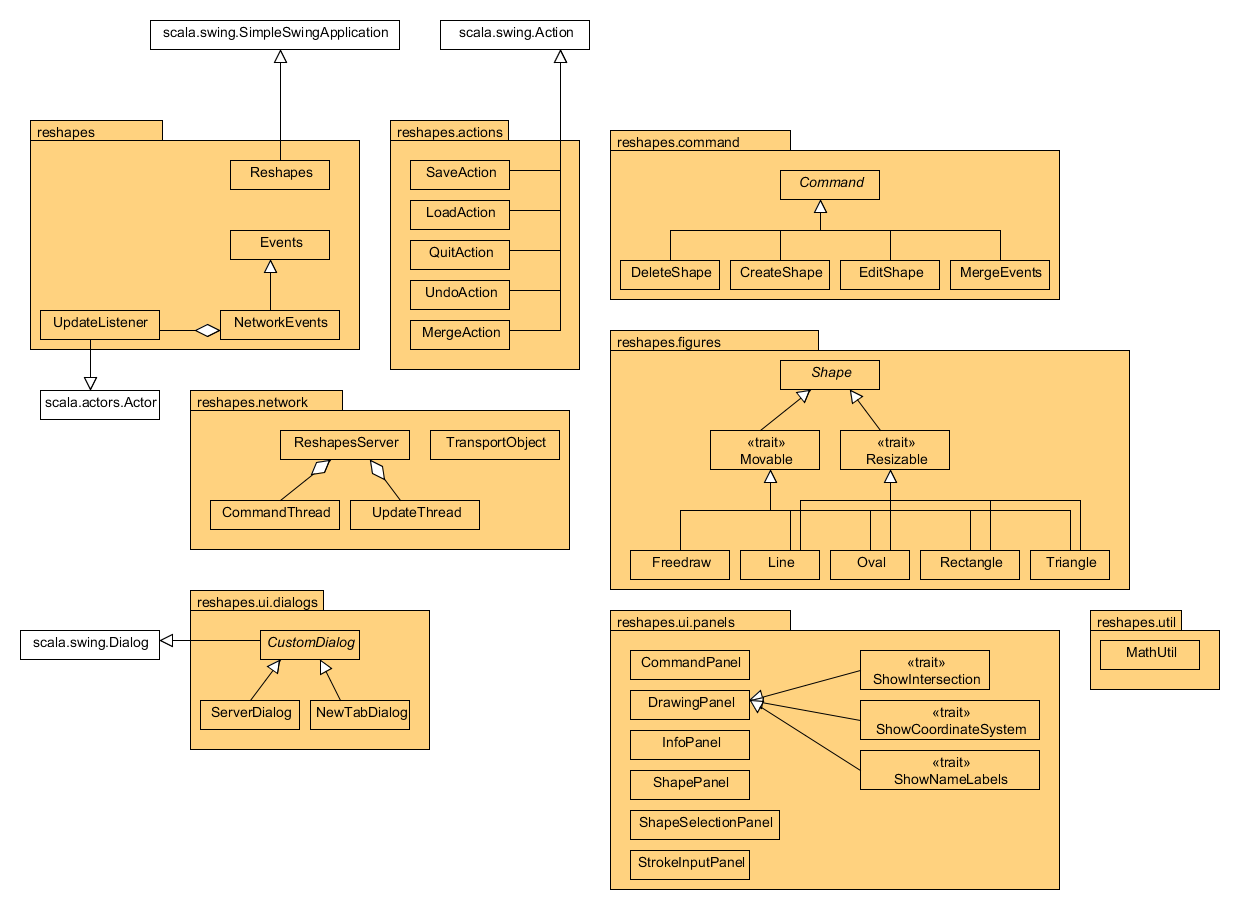
\includegraphics[width=1\textwidth]{img/class_diagram}

\section{Uses of EScala library}

The basis for all (EScala) events and signals is the class \textbf{reshapes.Events}: 

\fbox{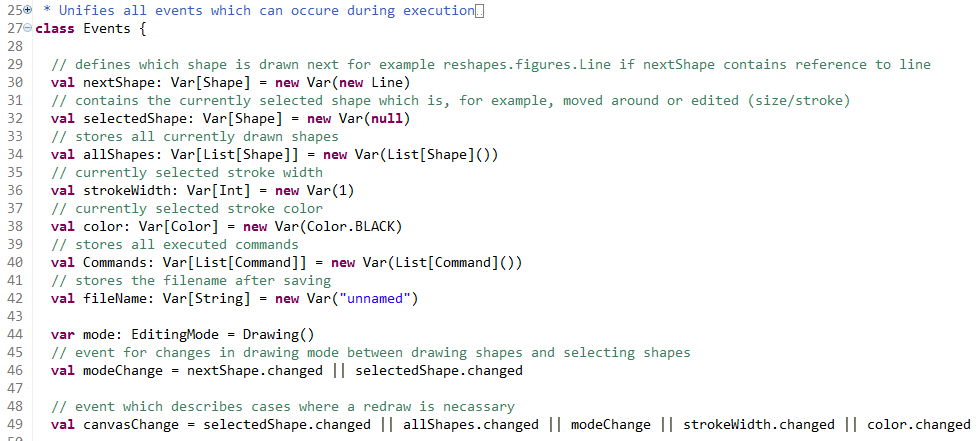
\includegraphics[width=1\textwidth]{img/events_class}}

This class defines all important variables as \textit{scala.events.behaviour.Var} on which different GUI and business logic parts of the application depend. 
Each tab/drawing pane has it own instance of \textit{Events}. \\
In the following subsections I will show which and how classes depend on these variables.

\subsection{reshapes.Events}

The \textit{Events} class itself adds four events: \\
\fbox{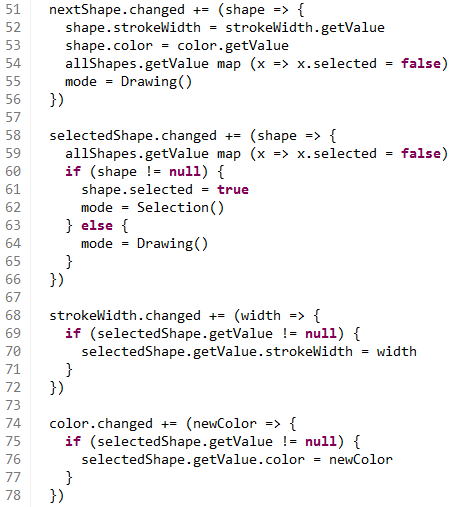
\includegraphics[width=.5\textwidth]{img/events_class_events}}

\subsection{reshapes.NetworkEvents}

\textit{NetworkEvents} is a subclass of \textit{Events}. 
Besides the responsibilities of \textit{Events} it adds the ability to send and receive updates to/from the server: \\
\fbox{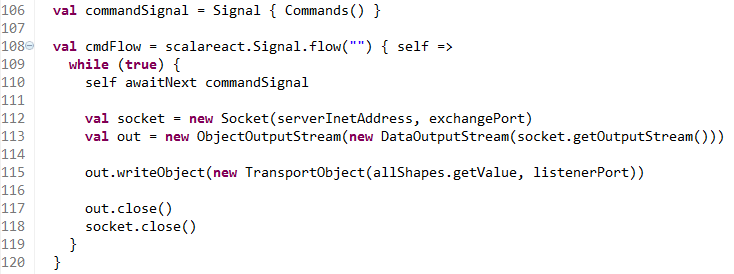
\includegraphics[width=.7\textwidth]{img/networkevents_events}} \\
What it does is, that it waits for changes in the command list and then sends all its currently drawn shapes to the server. 
I did not wait for changes in \textit{Events.allShapes} to prevent infinite updates.

\subsection{reshapes.Reshapes}

\textit{reshapes.Reshapes} holds a reference to the currently active \textit{Events} object (currently active drawing pane) and only defines one small \textit{Signal}: \\
\fbox{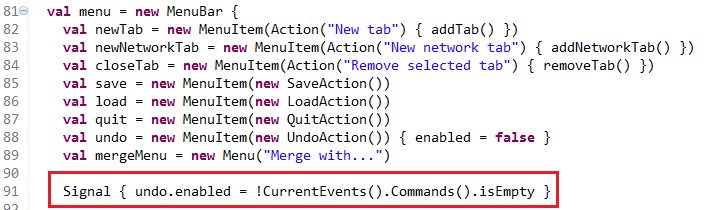
\includegraphics[width=.5\textwidth]{img/reshapes_events}} \\
Whenever commands are added/removed or the currently active tab changes it checks whether there are any commands left to undo. 
If not, the \textbf{Edit $\rightarrow$ Undo} menu item is disabled.

\subsection{reshapes.ui.panels.CommandPanel}

The \textit{CommandPanel} is the panel on the right side (when clicking on \textbf{Commands}). 
Like the \textit{Reshapes} object the signal evaluates when the active tab changes or commands are added/removed. \\
\fbox{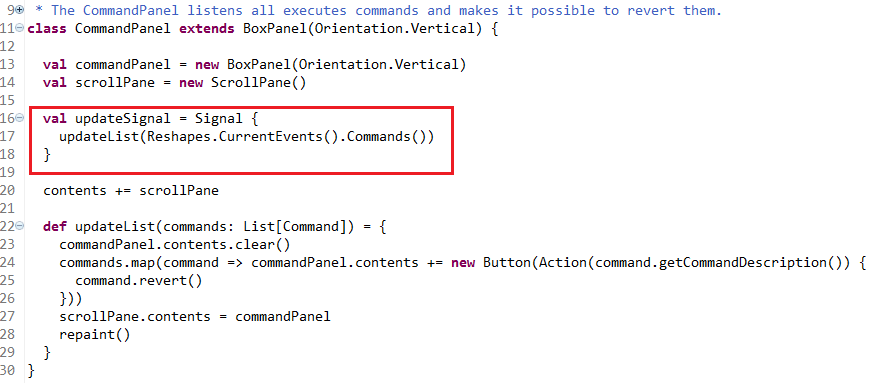
\includegraphics[width=1\textwidth]{img/commandpanel_events}}

\subsection{reshapes.ui.panels.DrawingPanel}

The \textit{DrawingPanel} is the main pane in the center of the application.
While the \textit{DrawingPanel} does a lot of stuff regarding drawing, keep track of mouse movements etc. this class only adds one event: \\
\fbox{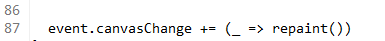
\includegraphics[width=.5\textwidth]{img/drawingpanel_events}} \\
This event is necassary to keep the displayed drawing up-to-date with the current status/underlying data structures.

\subsection{reshapes.ui.panels.InfoPanel}

The \textit{InfoPanel} is the small panel on the bottom.
The signals evaluates whenever the active tab changes or by changes of \textit{Events.nextShape, Events.selectedShape} and \textit{Events.allShapes}: \\
\fbox{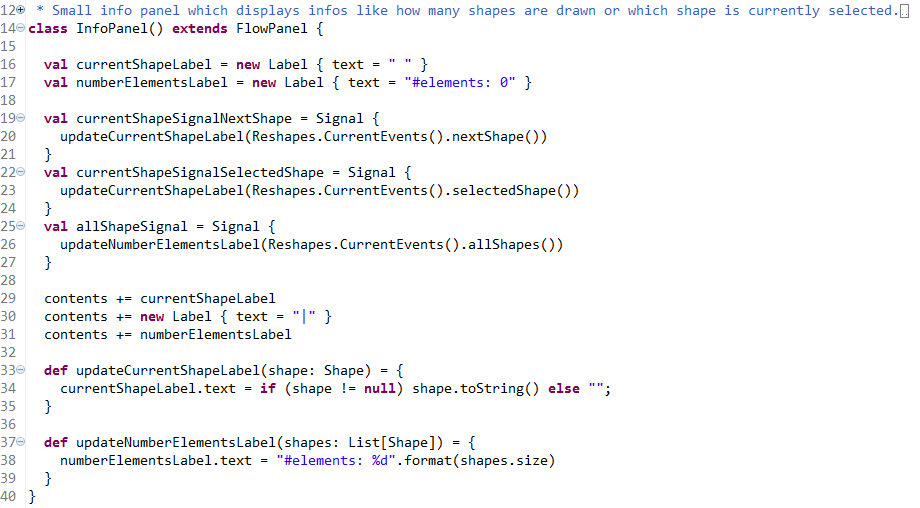
\includegraphics[width=1\textwidth]{img/infopanel_events}}

\subsection{reshapes.ui.panels.ShapePanel}

The \textit{ShapePanel} is on the right side showing all drawn shape in a list.
Because this panel highlights the selected shape it adds the following event: \\
\fbox{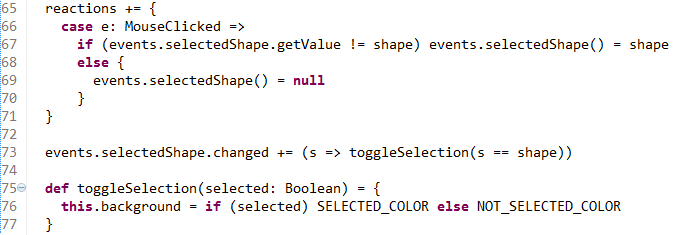
\includegraphics[width=.8\textwidth]{img/shapepanel_events}}

\section{Actions and their following event chain}

The following graphs shows some dependencies created with EScala. 
An edge with the label \textit{updates} means that the source node changes the content of the target node. 
Edges without labels mean that the target node is affected by the change of the source node (for example through signals).
Round nodes are attributes of classes (rectangle nodes).

\begin{figure}[h]
    \begin{center}
        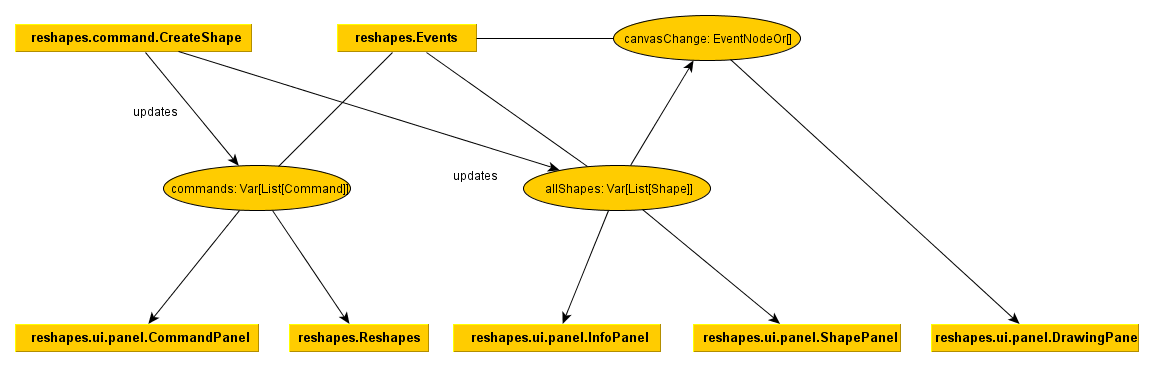
\includegraphics[width=1\textwidth]{img/createshape_events}
    \end{center}
    \caption{Dependencies when executing a CreateShape-Command}
    \label{fig:createshape_events}
\end{figure}

\begin{figure}[h]
    \begin{center}
        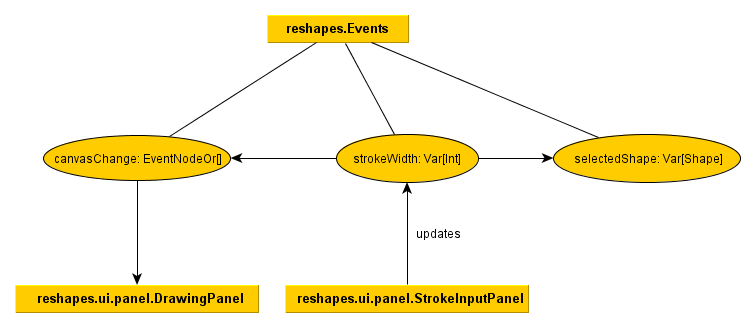
\includegraphics[width=1\textwidth]{img/strokeinput_events}
    \end{center}
    \caption{Changes of the stroke width}
    \label{fig:strokeinput_events}
\end{figure}

\begin{figure}[h]
    \begin{center}
        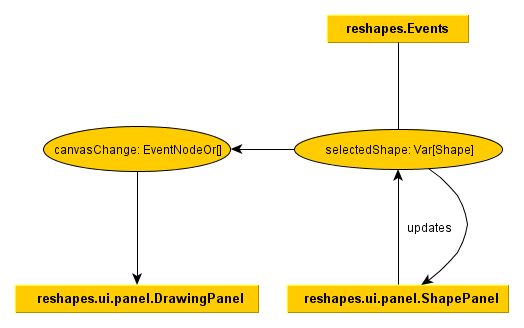
\includegraphics[width=1\textwidth]{img/shapeselect_events}
    \end{center}
    \caption{Dependencies when selecting a shape in the ShapePanel}
    \label{fig:shapeselect_events}
\end{figure}
